% Chapter Template

\chapter{Estudio de resistencia} % Main chapter title
\label{ChapterDESTRCCION}  % Change X to a consecutive number; for referencing this chapter elsewhere, use \ref{ChapterX}


Como se ha visto en el capítulo anterior, la estructura de la red mutualista determina la dinámica de poblaciones. El conjunto de interacciones es lo que mantiene la biodiversidad de los ecosistemas \cite{mccann2007protecting}.
Las propiedades de dicha estructura se resumen mediante indicadores estadísticos globales como el \textit{anidamiento}
y la \textit{modularidad}. Por su parte las medidas locales de centralidad y grado permiten ordenar las especies y conocer su importancia relativa para la resistencia de la red ante perturbaciones externas. 

Los índices que se manejan en la literatura son numerosos y de origen diverso y no existe un marco teórico que explique las relaciones entre los observables más habituales.

En este capítulo se describe el potencial de una técnica clásica en el análisis de grafos, conocida como \textit{descomposición k-core}, en el estudio de las redes mutualistas.

%----------------------------------------------------------------------------------------
%	SECTION 1
%----------------------------------------------------------------------------------------

\section{Propiedades estructurales del mutualismo}

Como se indicó en la introducción, la investigación sobre la estructura del mutualismo heredó las herramientas conceptuales del análisis de las \textit{food webs}, entre ellas el uso de la \textit{conectancia}. Esta magnitud es la fracción de enlaces presentes sobre todos los posibles entre las especies de ambas clases. En la actualidad resulta un índice global de utilidad limitada, pero sigue
usándose para la construcción de modelos nulos que veremos en este mismo capítulo. La distribución de grado es la traducción local de la conectancia,
y es muy heterogénea en las redes mutualistas, con algunas especies mucho más conectadas de lo que cabría esperar por azar \cite{jordano2003invariant}.

Durante la última década el \textit{anidamiento} se ha considerado como la característica distintiva del mutualismo\cite{bascompte2003nested}, aunque en la actualidad esta afirmación está sujeta a revisión. Este concepto tiene una definición clara en ecología, una comunidad es anidada si las especies encontradas en un ámbito geográfico reducido son un subconjunto de las existentes en un ámbito mayor más rico en recursos. Originalmente se aplicó al estudio de la distribución de la fauna en islas. La de una isla pequeña aislada es un subconjunto de la que existe en tierra firme o en una isla mayor de las mismas características biogeográficas \cite{young1958zoogeography, atmar1986nested}.

Si las especies se ordenan por grado, la matriz de interacción de una comunidad con anidamiento fuerte muestra abundancia de interacciones entre las especies situadas en el vértice superior izquierdo. Allí se concentran las muy conectadas,
las de grado reducido aparecen conectadas con este núcleo y raramente entre ellas .
\subsection{Algoritmo de destrucción basado en \textit{k-shell}}

Para poder establecer políticas de conservación es necesario disponer de un respaldo cuantitativo, localizando a las especies que más contribuyen a la estabilidad de las redes \cite{sole2001fragility, dakos2014resilience, thebault2010stability, suweis2013emergence, santamaria2015removing}.  Hay dos aproximaciones posibles. La primera se basa en la dinámica de ponlaciones y depende en gran medida de la parametrización del modelo elegido \cite{dakos2014critical}. La segunda, que utiliza solo la topología de la red, es más sencilla de implementar y por tanto mucho más popular. Es la que seguimos en este capítulo.

La biodiversidad y resistencia de una comunidad mutualista depende de su estructura. La extinción de algunas especies provoca que partes de la red queden desconectadas de la componente gigante y posiblemente expuestas a la desaparición. Por este motivo, la evolución del tamaño de la componente gigante cuando se eliminan especies es el criterio más utilizado para estudiar la resistencia estructural estática.

Esto es lo que hace el método de medida de Dunne \cite{dunne2002biodiversity}, ideado en origen para \textit{food webs}. Las especies se van retirando una por una de la red (extinciones primarias). Este hecho produce extinciones secundarias de aquellas especies. La gráfica de la fracción de la red inicial superviviente, frente a la fracción de extinciones primarias (en escala normalizada entre 0 y 1) define la \textit{curva de extinción}. Cuanto menor sea el área bajo esta curva, más rápida será la destrucción de la red.

\begin{figure}[h!]
\centering
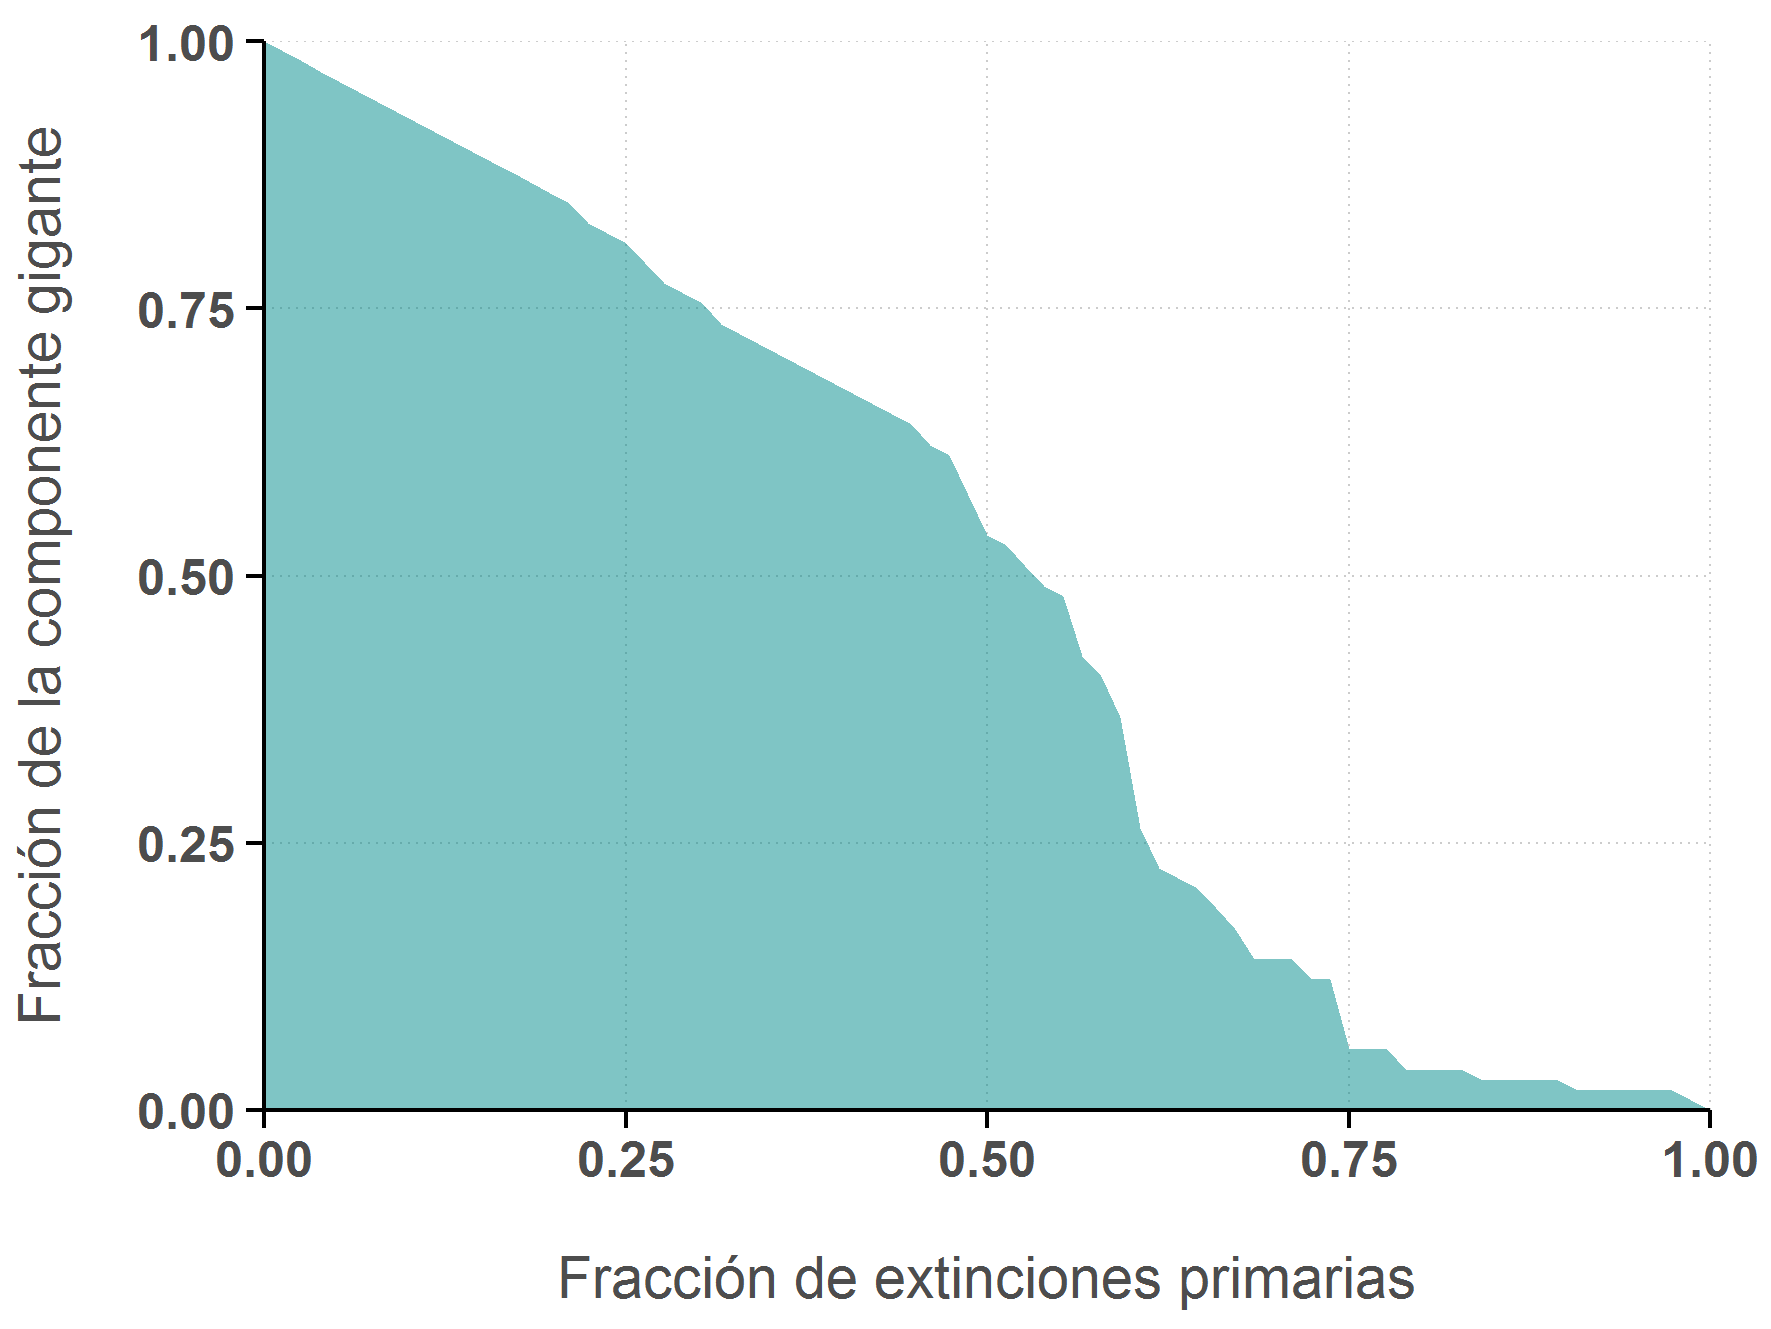
\includegraphics[scale=0.55]{Figures/ESTATICA_destruction_example.png}
\caption{Ejemplo de curva de extinción siguiendo el método de Dunne. El área bajo la curva indica la velocidad a la que se desintegra la componente gigante.}
\label{fig:ESTATICA_destruction_example}
\end{figure}

La clave está en el orden de selección de las especies que se retiran en las extinciones primarias. Si disponemos de una cifra que defina su importancia para esa red concreta, se podrán concentrar los esfuerzos de conservación en las especies que más aportan a la supervivencia del sistema. El problema es que no existe un criterio universalmente aceptado para establecer esa clasificación que resulte óptimo para cualquier red.

En el mutualismo, parece lógico pensar que las especies de las \textit{shells} más internas son las más importantes para mantener la integridad de la red. El algoritmo de destrucción que proponemos se basa en la secuencia $k$-$shell, k_{degree}, k_{radius}$, esto es, se empiezan las extinciones primarias por las especies pertenecientes a la $k$-$shell$ de mayor índice, y dentro de esta, el de mayor $k_{degree}$, y en caso de coincidencia, el de menor $k_{radius}$. 

\section{Material y métodos}

Para este capítulo hemos utilizado la colección de datos de redes mutualistas de la \textit{Web of Life}  \url{http://www.web-of-life.es/} \cite{fortuna2014web}. Hemos analizado todas las disponibles en las categorías \textit{planta-polinizador} y \textit{planta-dispersor de semillas}. En diciembre de 2015 dicha colección consta de 59 redes de la primera familia y 30 de la segunda. El número de especies por red varía entre 6 y 997 y el número de interacciones entre 6 y 2993.

El software se ha desarrollado en \texttt{R} y \texttt{Python}. La \textit{descomposición k-core} se realiza con el paquete \texttt{R} \texttt{igraph} \cite{csardi2006igraph}. El mismo paquete ofrece funciones para el cálculo de $NODF$ y $Modularity$. El código \texttt{R} para medir ${k}_{degree}$ y ${k}_{radius}$ es propio. Los valores medios de estas magnitudes se calculan descartando las especies que no pertenecen a la componente gigante cuando en la red se produce esta circunstancia. 

Para medir la bondad del algoritmo de destrucción, hemos comparado su rendimiento con el que ofrece \textit{MusRank}, de reciente publicación y basado en una clasificación de la importancia de los nodos similar a la del \textit{PageRank} de Google  \citep{dominguez2015ranking}. Tanto el algoritmo basado en \textit{k-shell} como la medición del \textit{MusRank} se han codificado en \texttt{Python}.



\subsection{Análisis mediante modelo nulo}
\label{sec:nullmodels}

El análisis de modelo nulo es una técnica para evaluar la significación estadística de las magnitudes de red y resulta imprescindible cuando estas no son libres de escala \cite{gotelli1996null}. En particular se ha aplicado en diversos trabajos para estudiar la validez de las distintas medidas de anidamiento \cite{ulrich2013pattern, feng2014heterogeneity} y modularidad \cite{fortuna2010nestedness, mello2011modularity}. En esta investigación se ha empleado para comparar el comportamiento de $\overline k_{radius}$ y de la medida de anidamiento $NODF$.

\section{Conclusiones}

La \textit{descomposición k-core} proporciona una sólida base para el análisis del mutualismo. Hemos demostrado como las \textit{k-magnitudes} definidas como propiedades surgidas del procedimiento, permiten conocer en detalle la estructura de las redes. En particular, al promediar los valores locales para todo el sistema, $\overline {k}_{radius}$ y $\overline {k}_{degree}$ muestran una fuerte correlación con los observables globales $NODF$ y $Modularity$. 

